\documentclass{article}
\usepackage{amsmath}
\usepackage{fancyhdr}
\usepackage{amsmath}
\usepackage{clrscode}
\usepackage{subfigure}
\usepackage[top=3cm, bottom=3cm, left=3cm, right=3cm]{geometry}
\usepackage[pdftex]{graphicx}\title{BME511L: Lab5}
\usepackage{float}
\usepackage{amsfonts}
\author{Allen Yin}
\pagestyle{fancy}
\setlength\parindent{0.0in}
\setlength\parskip{0.0in}
\usepackage{caption}
\captionsetup{justification=justified}
\setcounter{tocdepth}{2}
\setlength{\headheight}{15pt}

\begin{document}
\maketitle
\setlength\parskip{0.1in}

\section{Model 1: Lead Field}

The analytical formula for the lead potential and lead field, assuming a 2D, semi-infinite, homogeneous, and isotropic region is \[\Phi = -\frac{I_A}{\pi\sigma_0}ln{r_A}-\frac{I_B}{\pi\sigma_0}ln{r_B}\], and $\nabla{\Phi}$, respectively.

Plotted below are: a) Contour plot of the lead potential in a finite 2D tissue; b) Lead potentials for finite and semi-infinite regions, along the path L-R; c) x and y components of the lead fields for finite and semi-infinite regions, along the center of the path L-R.

\begin{figure}[H]
    \begin{center}
        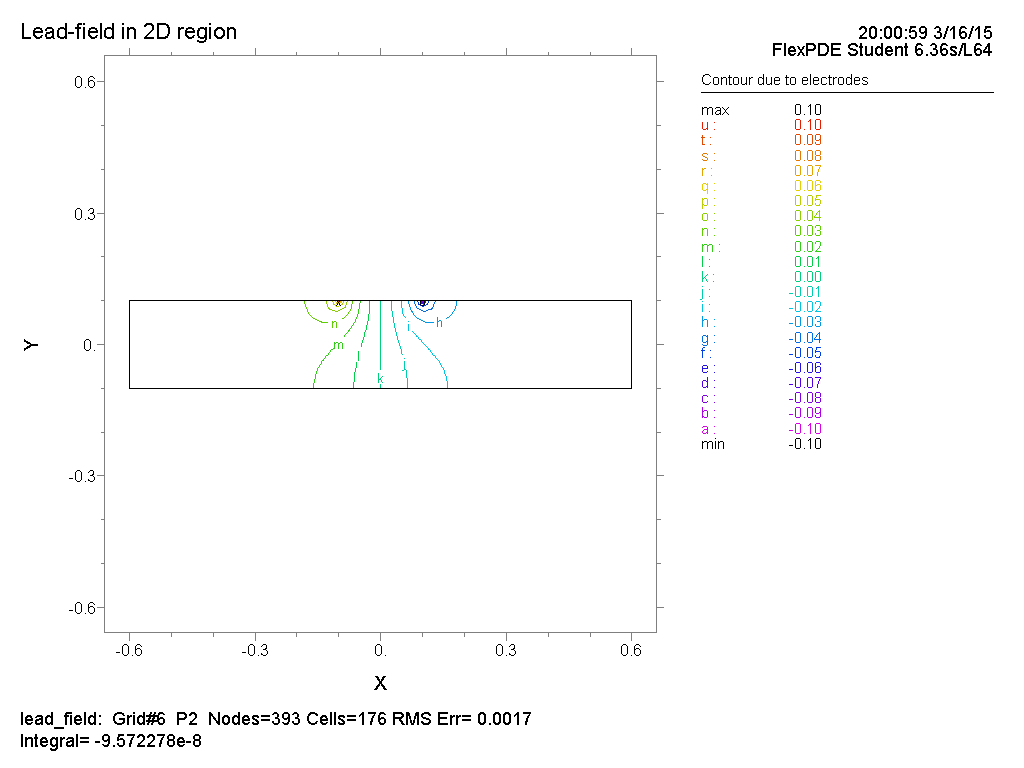
\includegraphics[scale=0.5]{lead_field_contour.png}
        \caption{Contour plot of the lead field. Electrode injects current on the left, and sinks current on the right.}
    \end{center}
\end{figure}

\begin{figure}[H]
    \begin{center}
        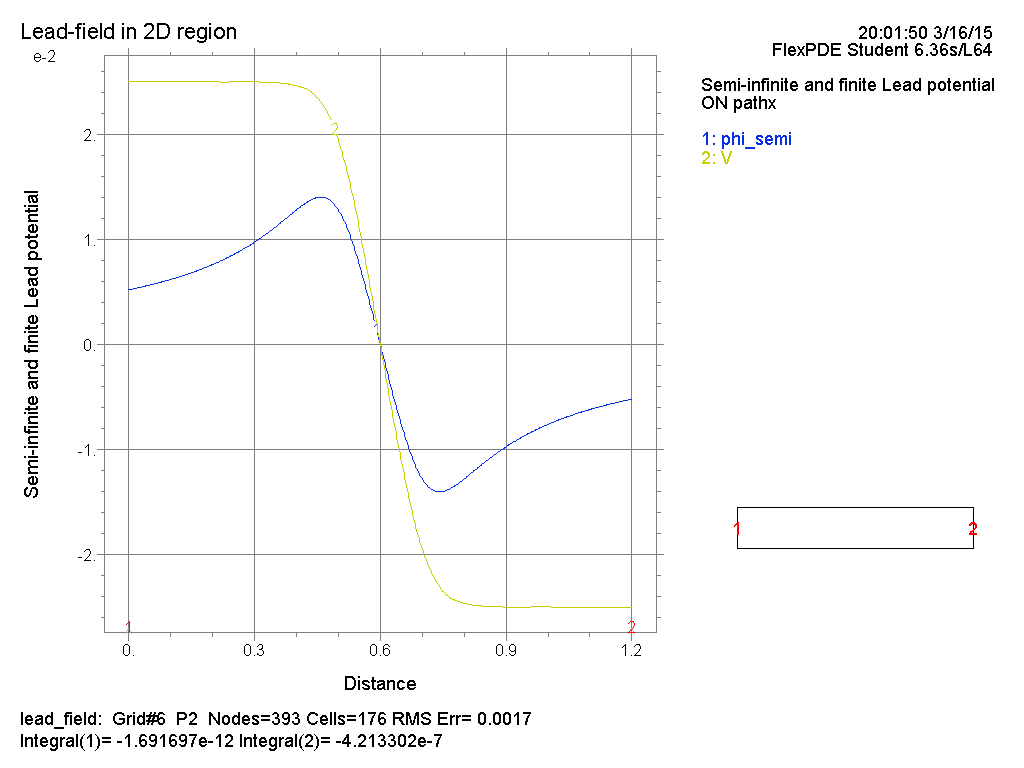
\includegraphics[scale=0.5]{lead_potential.png}
        \caption{Lead potentials $\Phi$ for finite and semi-infinite regions, plotted together along the path L-R. Yellow is for finite region. Blue is for semi-infinite region.}
    \end{center}
\end{figure}

\begin{figure}[H]
    \begin{center}
        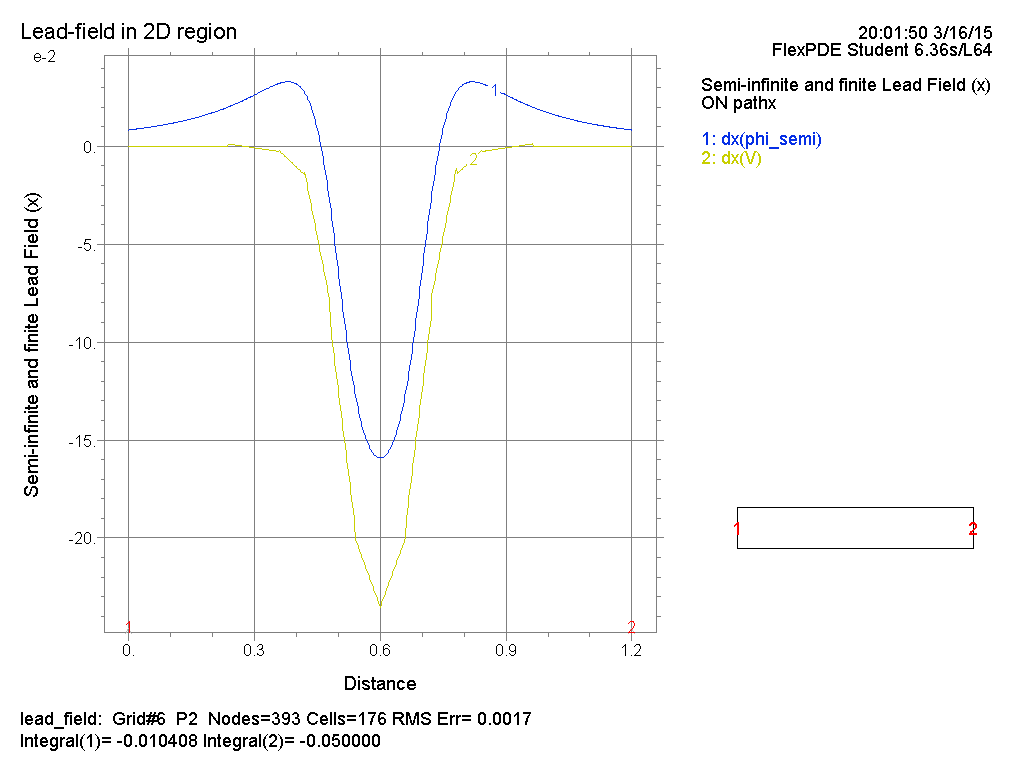
\includegraphics[scale=0.5]{lead_field_x.png}
        \caption{The x-component of the Lead field, $\nabla \Phi_x$ for finite and semi-infinite regions, plotted together along the path L-R. Yellow is for finite regions. Blue is for semi-infinite region.}
    \end{center}
\end{figure}

\begin{figure}[H]
\begin{center}
        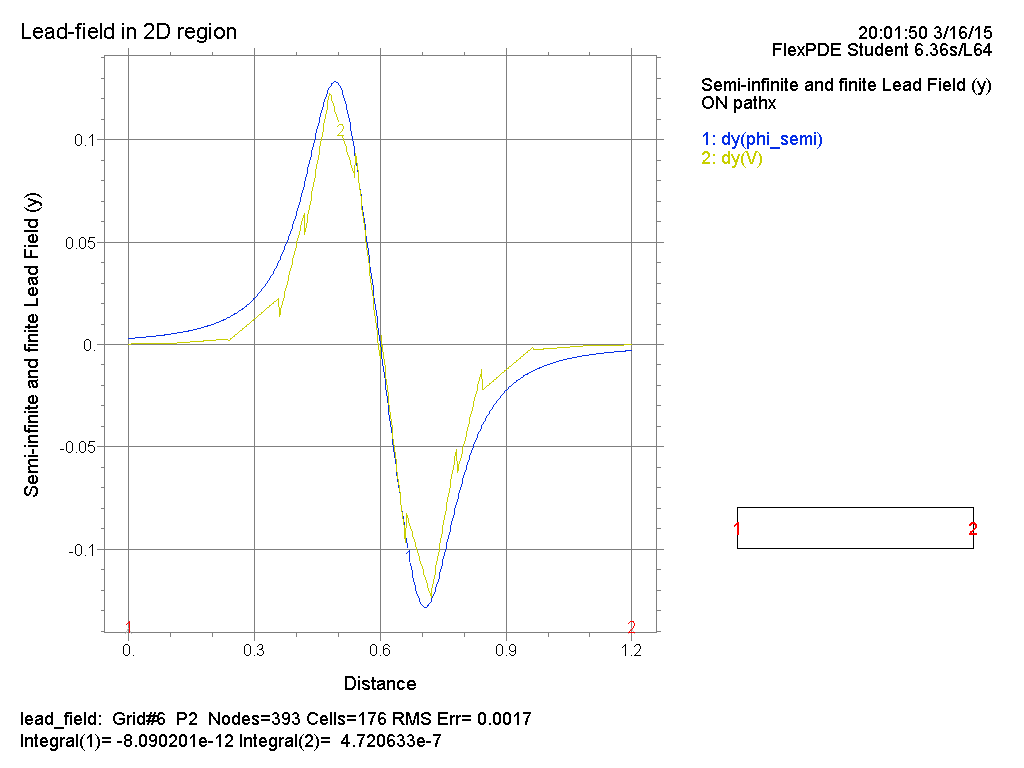
\includegraphics[scale=0.5]{lead_field_y.png}
        \caption{The y-component of the Lead field, $\nabla \Phi_y$ for finite and semi-infinite regions, plotted together along the path L-R. Yellow is for finite regions. Blue is for semi-infinite region.}
    \end{center}
\end{figure}

\section{Model 2: Active Fiber and Measured Voltage}
In flexPDE, we compute the voltage measured by the two electrodes via reciprocity theorem by the integral \[V_{AB} = \int_V \mathbf{J_i}\cdot\nabla\phi_2dv\], where the integral is taken over the fiber volume $V$, $\mathbf{J_i}$ is the intracellular current in the bidomain model: \[\mathbf{J_i} = -\frac{g_ig_e}{g_i+g_e}\nabla V_m\], and $\nabla\phi_2$ is the lead field computed from the previous section. 

This voltage $V_{AB}$ is computed as a function of time, as $V_m$ changes according to the propagating action potential from $t=0ms$ to $t=15ms$. The transmembrane potential $V_m$ and that measured at the electrodes $V_{AB}$, for a fiber in both finite and semi-infinite regions are plotted below.

\begin{figure}[H]
    \begin{center}
        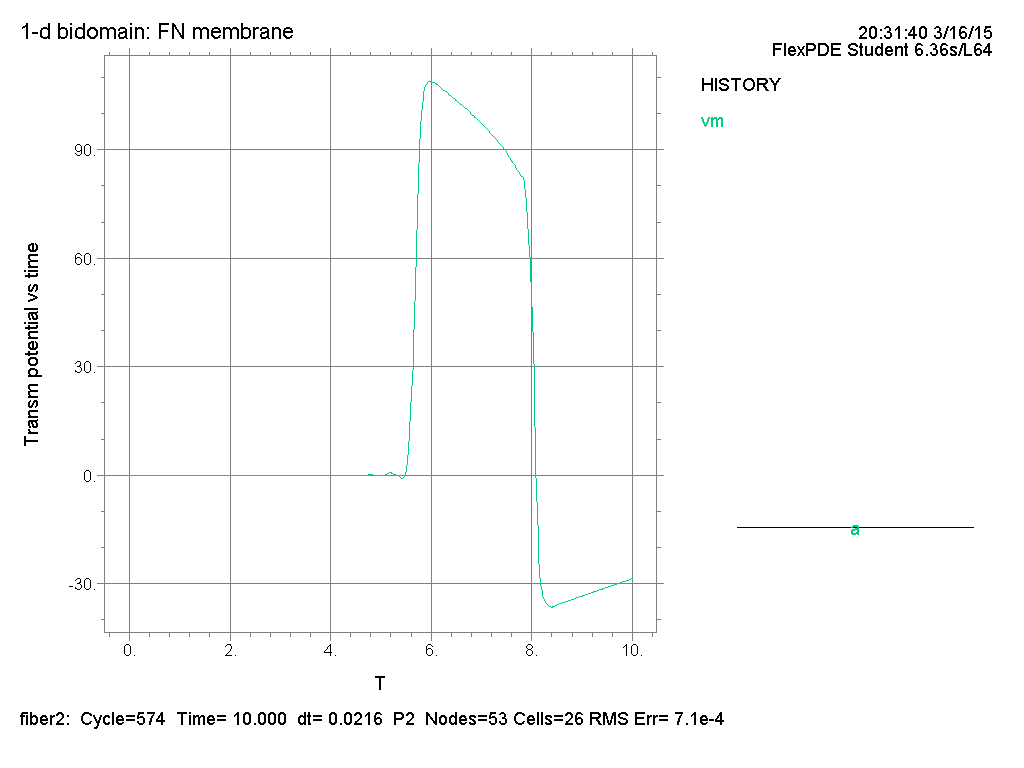
\includegraphics[scale=0.5]{fiber2_Vm.png}
        \caption{Transmembrane potential $V_m$ over time, at the middle of the fiber}
    \end{center}
\end{figure}

\begin{figure}[H]
    \begin{center}
        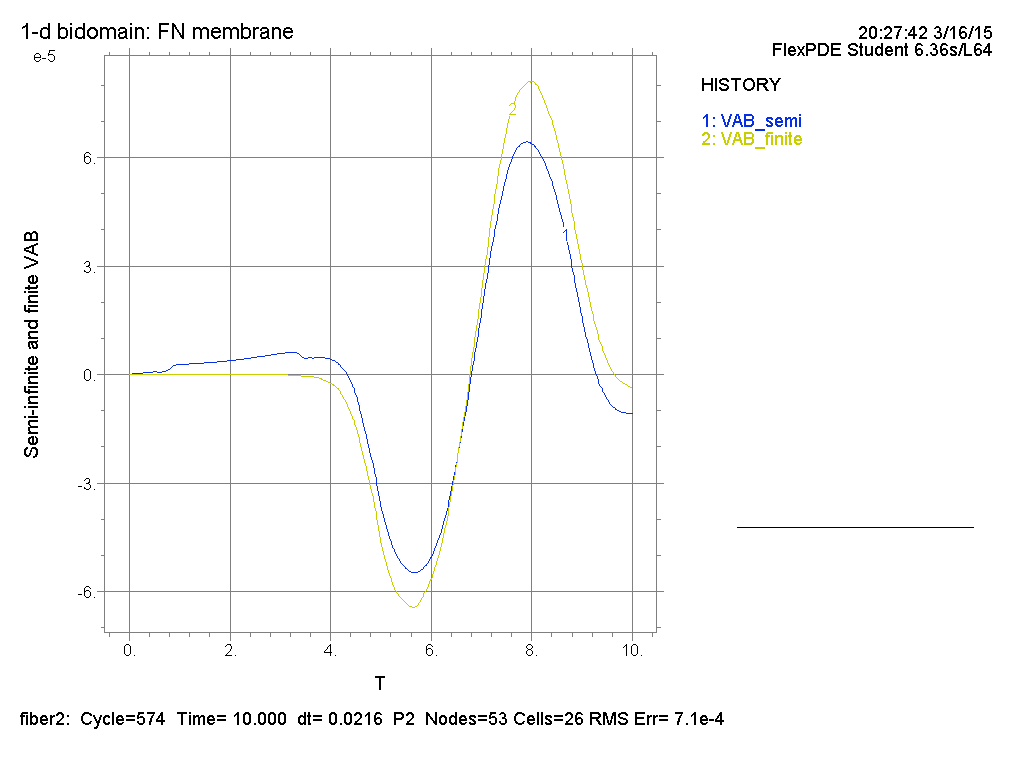
\includegraphics[scale=0.5]{fiber2_VAB.png}
        \caption{Voltage measured at the surface electrodes, $V_{AB}$, computed as a function of time via the reciprocity principle. Yellow is that in a finite region. Blue is that in a semi-infinite region.}
    \end{center}
\end{figure}

\section{Discussion}

\subsection{Lead Potentials and Lead Fields}
As seen in Figure 2, the lead potential in a semi-infinite region has the same value as in the finite region at x=0. This is neccessitated by the boundary condition set at $x=0$. The lead potential curves also have the same general shape. However, in the semi-infinite region, the absolutel potentials peak at the same position as in the finite region, but at a lower magnitude, and then proceeds to decay further away from the electrodes. This is in contrast with the finite region lead-potential, where once reaching the peak, the lead potential remains flat. 

This difference occurs because in the finite region, there is a no-flux boundary condition around the entire region except for the electrodes. Thus the entire potential change in the finite case happens between the two electrodes, so we see no potential change beyond the electrode positions. In semi-infinite region, however, flux lines are free to go in any directions, resulting in the decay away from the electrode positions.

This is also the reason why, in Figure 3,  we see a greater magnitude in the lead-field for the finite region, and decay of the lead-field away from the electrode positions for the semi-infinite region.

\subsection{$V_{AB}$}
$V_{AB}$ measured in finite region and semi-infinite region are pretty similar, showing a negative peak followed by a positive peak. The big difference is that preceeding the first negative peak, the potential measured in the semi-infinite region rises up slightly, while the potential measured in the finite region stays flat.

This is because in the semi-infinite region, flux around the boundary is nonzero. Thus, more of the fiber contribute to the voltage measurement, resulting in a slow build up to the peak. In other words, field lines from the fiber can reach the electrodes in more ways than in the finite region case.  Mathematically, as seen in Figure 3, the lead-field for the semi-infinite region is nonzero for the entire fiber, thus the product within the integral for $V_{AB}$ is nonzero for a longer time range, resulting in the slow rise in measured $V_{AB}$.

We see some glitches/artifacts in the $V_{AB}$ for the semi-infinite case because of the approximations we have made in deriving the analytical solution used to calculate the lead field.

\end{document}
